\begin{align}
\bF_t &= \balpha S(C_t + \beta) +  \ve{\varepsilon}_t, \qquad &\ve{\varepsilon}_t \sim \mathcal{N}(\ve{0},\sig^2 \bI)
\end{align}

\noindent where $S(x)=\frac{x^{n_d}}{x^{n_d}+k_d}$

note: initialize with linear result, but add a constant wherever constraint is not satisfied

\begin{figure}[H]
%\centering 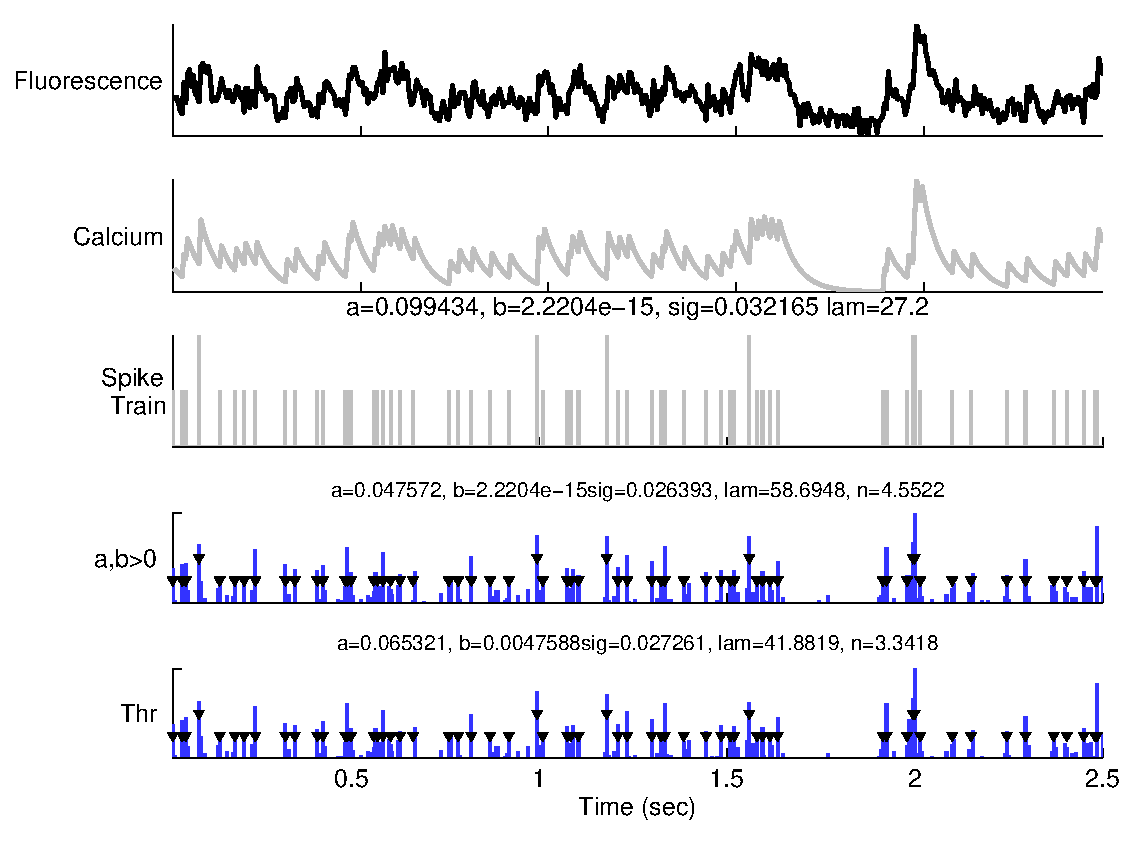
\includegraphics[width=.9\linewidth]{schem}
\caption{Saturation} \label{fig:satur}
\end{figure}
